\section{Auswertung}
\label{sec:Auswertung}

\subsection{Bestätigung des Linsengesetzes}

Bei der ersten Messung wurden $g$, $b$ und $B$ bestimmt. Unter Verwendung des Linsengesetzes 
kann zunächst $\frac{1}{f}$ und schließlich $f$ bestimmt werden. Für die Linse bekannter
Brennweite ($\SI{0.150}{\meter}$) ergibt sich somit Tabelle \ref{tab:mess1}. Das Abbildungsgesetz 
kann überprüft werden, indem für jeden Messwert $V_1 = \frac{b}{g}$ und $V_2= \frac{B}{G}$
bestimmt wird. Weiter wird die Differenz $\vert\Delta V \vert$ berechnet. Hierbei erkennt 
man, dass diese Differenz für jeden der Messwerte bei der Linse sehr klein ist.\\

\begin{table}
    \centering
    \caption{Messwerte und Brennweite der Linse mit bekannter Brennweite.}
    \label{tab:mess1}
    \sisetup{table-format=2.1}
    \begin{tabular}{c c c c c c c}
    \toprule
    $ g \;/\; \si{\meter} $ & $b \;/\; \si{\meter}$ &
    $ B \;/\; \si{\meter} $ & $V_1$ & $V_2$ & $\vert \Delta V \vert$ & $f \;/\; \si{meter}$\\
    \midrule 
        0,25 & 0,465 & 0,0450 & 1,860 & 1,500 & 0,360 & 0.163\\
        0,30 & 0,356 & 0,0260 & 1,867 & 0,867 & 0,320 & 0.163\\
        0,35 & 0,300 & 0,0190 & 0,857 & 0,633 & 0,224 & 0.162\\
        0,40 & 0,277 & 0,0160 & 0,693 & 0,533 & 0,159 & 0.164\\
        0,45 & 0,257 & 0,0125 & 0,571 & 0,417 & 0,154 & 0.164\\
        0,50 & 0,243 & 0,0110 & 0,486 & 0,367 & 0,119 & 0.164\\
        0,55 & 0,233 & 0,0095 & 0,424 & 0,317 & 0,107 & 0.164\\
        0,60 & 0,226 & 0,0080 & 0,377 & 0,267 & 0,110 & 0.164\\
        0,65 & 0,218 & 0,0070 & 0,335 & 0,233 & 0,102 & 0.163\\
        0,70 & 0,205 & 0,0065 & 0,293 & 0,217 & 0,076 & 0.159\\          
    \bottomrule
    \end{tabular}
    \end{table}

Aus Tabelle \ref{ta:mess1} folgt somit für den Brennpunkt $f$ als Mittelwert 

\begin{equation*}
\SI{0.163+-0.002}{\meter}.
\end{equation*}

Werden die Wertepaare $(g_i, b_i)$ auf die Achsen eines Koordinatensystems aufgetragen, und 
die zugehören Paare miteinander verbunden, so ergibt sich für die Linse bekannter 
Brennweite Abbildung \ref{fig:plot1}.

\begin{figure}
  \centering
  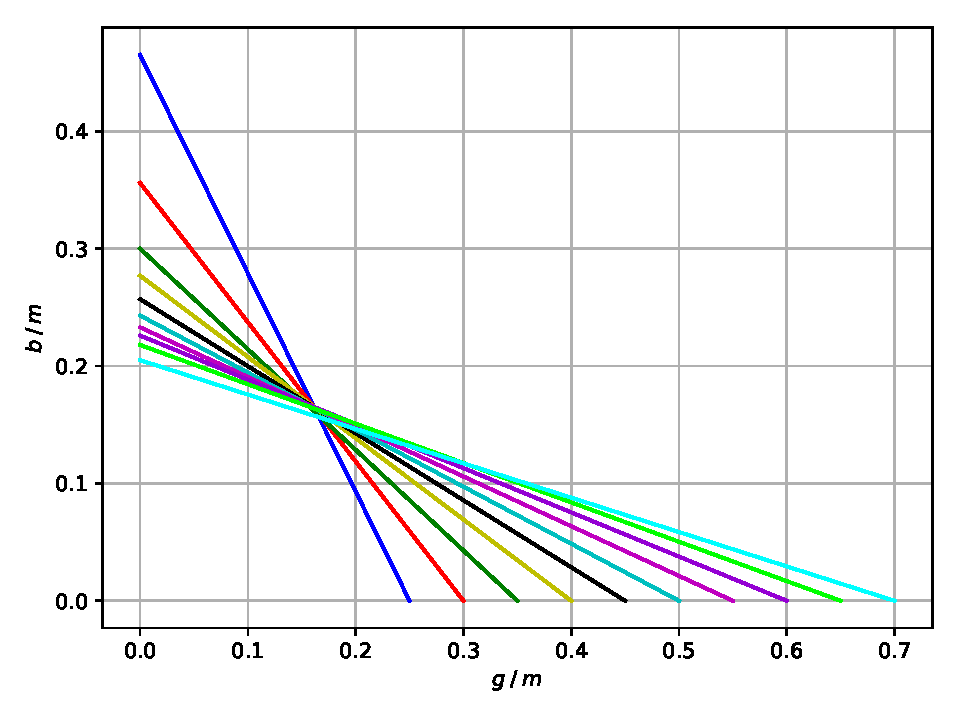
\includegraphics{content/plot1.pdf}
  \caption{Wertepaare f bekannt.}
  \label{fig:plot1}
\end{figure}

Es ein Ausreißer zu erkennen (cyan Gerade), der beim Ablesen der Brennweite außer Acht gelassen wird. 
Der Schnittpunkt aller Geraden der Messwerte bestimmt den Brennpunkt $f$ der Linse. Dieser
Schnittpunkt wird so genau wie möglich abgelesen. Es ergibt sich der Punkt 

\begin{equation*}
(\SI{0.16}{meter} \vert \SI{0.16}{\meter}).
\end{equation*}

und da die beiden Werte gleich sind, ergibt sich 

\begin{equation*}
f = \SI{0.16}{\meter}.
\end{equation*}

\subsection{Methode von Bessel}

Bei der zweiten Messung wurden die beiden Positionen mit scharfem Bild für ungefiltertes, 
blaues und rotes Licht nach der Methode nach Bessel bestimmt. Aus diesen Messwerten lässt 
sich nach Formel \eqref{eqn:bessel} die Brennweite der Linse bestimmen. Alles Messwerte, sowie die für die
einzelne Messwerte berechneten Brennweiten sind in Tabelle \ref{tab:mess2}, 
\ref{tab:mess3} und \ref{tab:mess4} dargestellt. 

\begin{table}
    \centering
    \caption{Besselmethode ungefiltertes Licht.}
    \label{tab:mess2}
    \sisetup{table-format=2.1}
    \begin{tabular}{c c c c c c c c c}
    \toprule
    $ e \;/\; \si{\meter} $ & $g_1 \;/\; \si{\meter}$ &
    $ b_1 \;/\; \si{\meter}$ & $g_2 \;/\; \si{\meter}$ & 
    $ b_2 \;/\; \si{\meter}$ & $\vert g_1 - b_1 \vert$ & 
    $ \vert g_2 - b_2 \vert$ & $ f_1 \;/\; \si{\meter}$ &
    $ f_2 \;/\; \si{\meter}$\\
    \midrule 
        0,900 & 0,2120 & 0,6880 & 0,687 & 0,213 & 0,476 & 0,474 & 0,162 & 0,163\\
        0,850 & 0,2170 & 0,6330 & 0,632 & 0,218 & 0,416 & 0,414 & 0,162 & 0,162\\
        0,820 & 0,2240 & 0,5960 & 0,598 & 0,222 & 0,372 & 0,376 & 0,163 & 0,162\\
        0,800 & 0,2270 & 0,5730 & 0,572 & 0,228 & 0,346 & 0,344 & 0,163 & 0,163\\
        0,770 & 0,2310 & 0,5390 & 0,532 & 0,238 & 0,308 & 0,294 & 0,162 & 0,164\\
        0,750 & 0,2365 & 0,5135 & 0,510 & 0,240 & 0,277 & 0,270 & 0,162 & 0,163\\
        0,720 & 0,2470 & 0,4730 & 0,468 & 0,252 & 0,226 & 0,216 & 0,162 & 0,164\\
        0,700 & 0,2550 & 0,4450 & 0,445 & 0,255 & 0,190 & 0,190 & 0,162 & 0,162\\
        0,675 & 0,2720 & 0,4030 & 0,402 & 0,273 & 0,131 & 0,129 & 0,162 & 0,163\\
        0,650 & 0,3070 & 0,3430 & 0,352 & 0,298 & 0,036 & 0,054 & 0,162 & 0,161\\          
    \bottomrule
    \end{tabular}
    \end{table}

\begin{table}
    \centering
    \caption{Besselmethode rotes Licht.}
    \label{tab:mess3}
    \sisetup{table-format=2.1}
    \begin{tabular}{c c c c c c c c c}
    \toprule
    $ e \;/\; \si{\meter} $ & $g_1 \;/\; \si{\meter}$ &
    $ b_1 \;/\; \si{\meter}$ & $g_2 \;/\; \si{\meter}$ & 
    $ b_2 \;/\; \si{\meter}$ & $\vert g_1 - b_1 \vert$ & 
    $ \vert g_2 - b_2 \vert$ & $ f_1 \;/\; \si{\meter}$ &
    $ f_2 \;/\; \si{\meter}$\\
    \midrule 
        0,90 & 0,214 & 0,686 & 0,683 & 0,217 & 0,472 & 0,466 & 0,163 & 0,165\\
        0,85 & 0,220 & 0,630 & 0,627 & 0,223 & 0,410 & 0,404 & 0,163 & 0,164\\
        0,80 & 0,228 & 0,572 & 0,570 & 0,230 & 0,344 & 0,340 & 0,163 & 0,164\\
        0,75 & 0,240 & 0,510 & 0,509 & 0,241 & 0,270 & 0,268 & 0,163 & 0,164\\
        0,70 & 0,261 & 0,439 & 0,442 & 0,258 & 0,178 & 0,184 & 0,164 & 0,163\\         
    \bottomrule
    \end{tabular}
    \end{table}

\begin{table}
    \centering
    \caption{Besselmethode blaues Licht.}
    \label{tab:mess4}
    \sisetup{table-format=2.1}
    \begin{tabular}{c c c c c c c c c}
    \toprule
    $ e \;/\; \si{\meter} $ & $g_1 \;/\; \si{\meter}$ &
    $ b_1 \;/\; \si{\meter}$ & $g_2 \;/\; \si{\meter}$ & 
    $ b_2 \;/\; \si{\meter}$ & $\vert g_1 - b_1 \vert$ & 
    $ \vert g_2 - b_2 \vert$ & $ f_1 \;/\; \si{\meter}$ &
    $ f_2 \;/\; \si{\meter}$\\
    \midrule 
        0,90 & 0,212 & 0,688 & 0,687 & 0,213 & 0,476 & 0,474 & 0,162 & 0,163\\
        0,85 & 0,218 & 0,632 & 0,631 & 0,219 & 0,414 & 0,412 & 0,162 & 0,163\\
        0,80 & 0,227 & 0,573 & 0,572 & 0,226 & 0,346 & 0,346 & 0,163 & 0,163\\
        0,75 & 0,236 & 0,514 & 0,511 & 0,239 & 0,278 & 0,272 & 0,162 & 0,163\\
        0,70 & 0,250 & 0,445 & 0,442 & 0,258 & 0,195 & 0,184 & 0,161 & 0,163\\         
    \bottomrule
    \end{tabular}
\end{table}

Aus diesen Tabellen ergeben sich als Mittelwerte für die Brennweiten

\begin{align*}
f &= \SI{0.1621+-0.0003}{\meter},\\
f_\text{rot} &= \SI{0.1639+-0.0006}{\meter},\\
f_\text{blau} & = \SI{0.1627+-0.0001}{\meter}.
\end{align*}

\subsection{Methode von Abbe}
Bei der dritten Messung soll die Brennweite, sowie die Positionen der Hauptebene eines Linsensystems 
bestimmt werden. Aus den gemessen Werten für $B$ lässt sich der Abbildungsmaßstab $V$ bestimmen. Daraus 
wiederum lassen sich die Größen $(1+\frac{1}{V})$ und $(1+V)$ berechnen. Diese Größen sind 
in Tabelle \ref{tab:mess5} eingetragen.

\begin{table}
    \centering
    \caption{Messwerte Methode nach Abbe}
    \label{tab:mess5}
    \sisetup{table-format=2.1}
    \begin{tabular}{c c c c c c}
    \toprule
    $ g' \;/\; \si{\meter} $ & $b' \;/\; \si{\meter}$ &
    $ B \;/\; \si{\meter} $ & $V$ & $1+\frac{1}{V}$ & $1+V$\\
    \midrule 
        0,20 & 0,740 & 0,0570 & 1,90 & 1,526 & 2,90\\
        0,25 & 0,555 & 0,0340 & 1,13 & 1,882 & 2,13\\
        0,30 & 0,470 & 0,0230 & 0,77 & 2,304 & 1,77\\
        0,35 & 0,433 & 0,0180 & 0,60 & 2,667 & 1,60\\
        0,40 & 0,395 & 0,0190 & 0,63 & 2,579 & 1,63\\
        0,45 & 0,385 & 0,0120 & 0,40 & 3,500 & 1,40\\
        0,47 & 0,372 & 0,0125 & 0,42 & 3,400 & 1,42\\
        0,50 & 0,370 & 0,0100 & 0,33 & 4,000 & 1,33\\
        0,55 & 0,353 & 0,0090 & 0,30 & 4,333 & 1,30\\
        0,60 & 0,350 & 0,0080 & 0,27 & 4,750 & 1,37\\          
    \bottomrule
    \end{tabular}
    \end{table}

Weiter wird $g'$ gegen $(1+1/V)$ und $b'$ gegen $(1+V)$ aufgetragen, woraus Abbildung \ref{fig:plot2}
und \ref{fig:plot3} resultieren.  

\begin{figure}
  \centering
  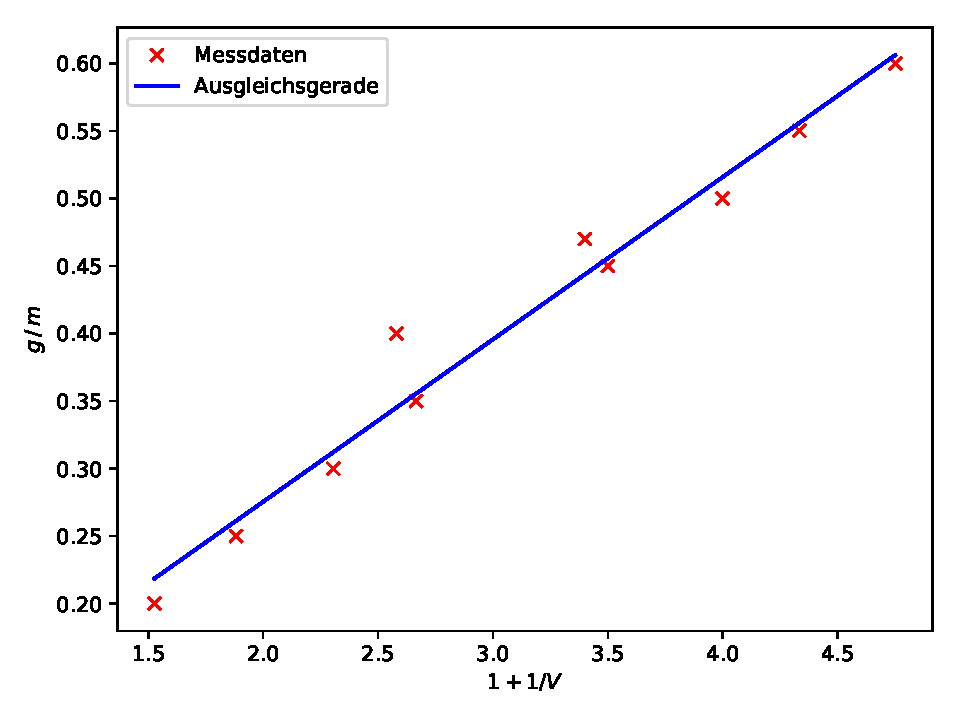
\includegraphics{content/plot2.pdf}
  \caption{Messwerte $g'$ gegen $1+1/V)$.}
  \label{fig:plot2}
\end{figure}

\begin{figure}
  \centering
  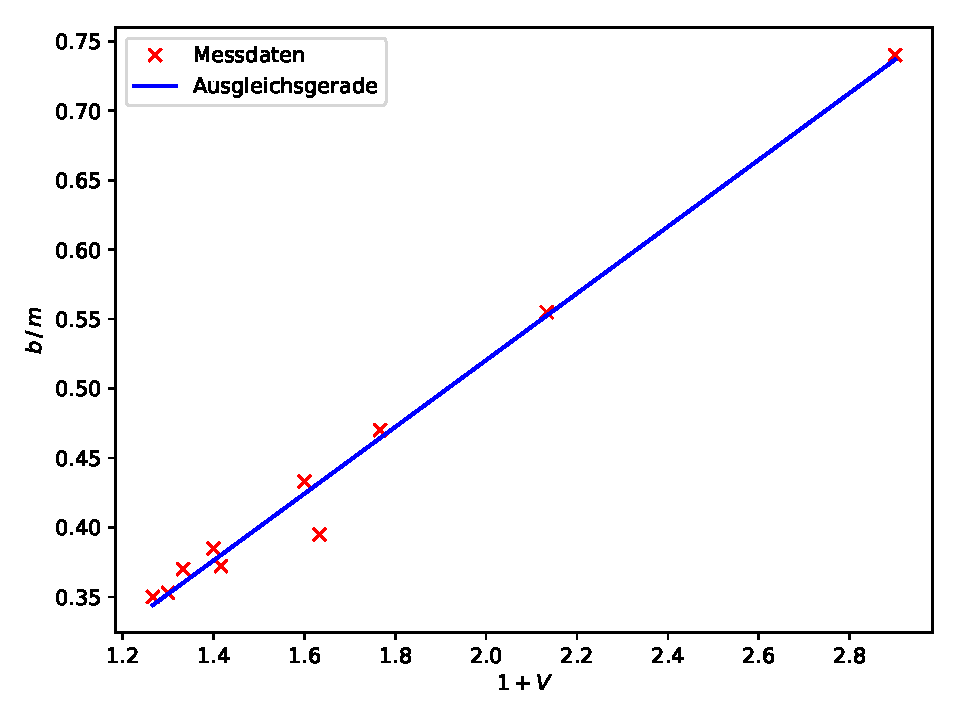
\includegraphics{content/plot3.pdf}
  \caption{Messwerte $b'$ gegen $1+V$.}
  \label{fig:plot3}
\end{figure}

Es wurde jeweils eine lineare Regression mittels Python durchgeführt. Die dabei erhaltenen Parameter 
geben hierbei nach Formel \eqref{eqn:abbe1} und \eqref{eqn:abbe} direkt den Brennpunkt und die Lage der Hauptebenen an. Es ergibt sich
für 

\begin{align*}
g' &= g + h = f_1 \cdot \left(1+\frac{1}{V}\right)+h,\\
b' &= b + h = f_2 \cdot \left(1+V\right)+h'  
\end{align*}

und somit 

\begin{align*}
f_1 &= \SI{0.120+-0.009}{\meter}, \\
f_2 &= \SI{0.240+-0.011}{\meter}, \\
h & = \SI{0.035+-0.028}{\meter},\\
h'&= \SI{0.040+-0.020}{\meter}.
\end{align*}

Es ist erkennbar, dass $f_1$ und $f_2$ nicht denselben Wert besitzen, sodass für die letztliche 
Bestimmung der Brennweite der Mittelwert gebildet wird. Es folgt somit

\begin{equation*}
f = \SI{0.180+-0.060}{\meter}.
\end{equation*}

Die Position der Hauptebenen $h$ und $h'$ beziehen sich auf den Referenzpunkt $A$. Dieser hat gerade die 
Mittelebene der dünnen Sammellinse. 